\documentclass{standalone}
\usepackage{tikz}
\usetikzlibrary{patterns, positioning}
\usepackage[sfdefault]{ClearSans} %% option 'sfdefault' activates Clear Sans as the default text font
\usepackage[T1]{fontenc}

\begin{document}
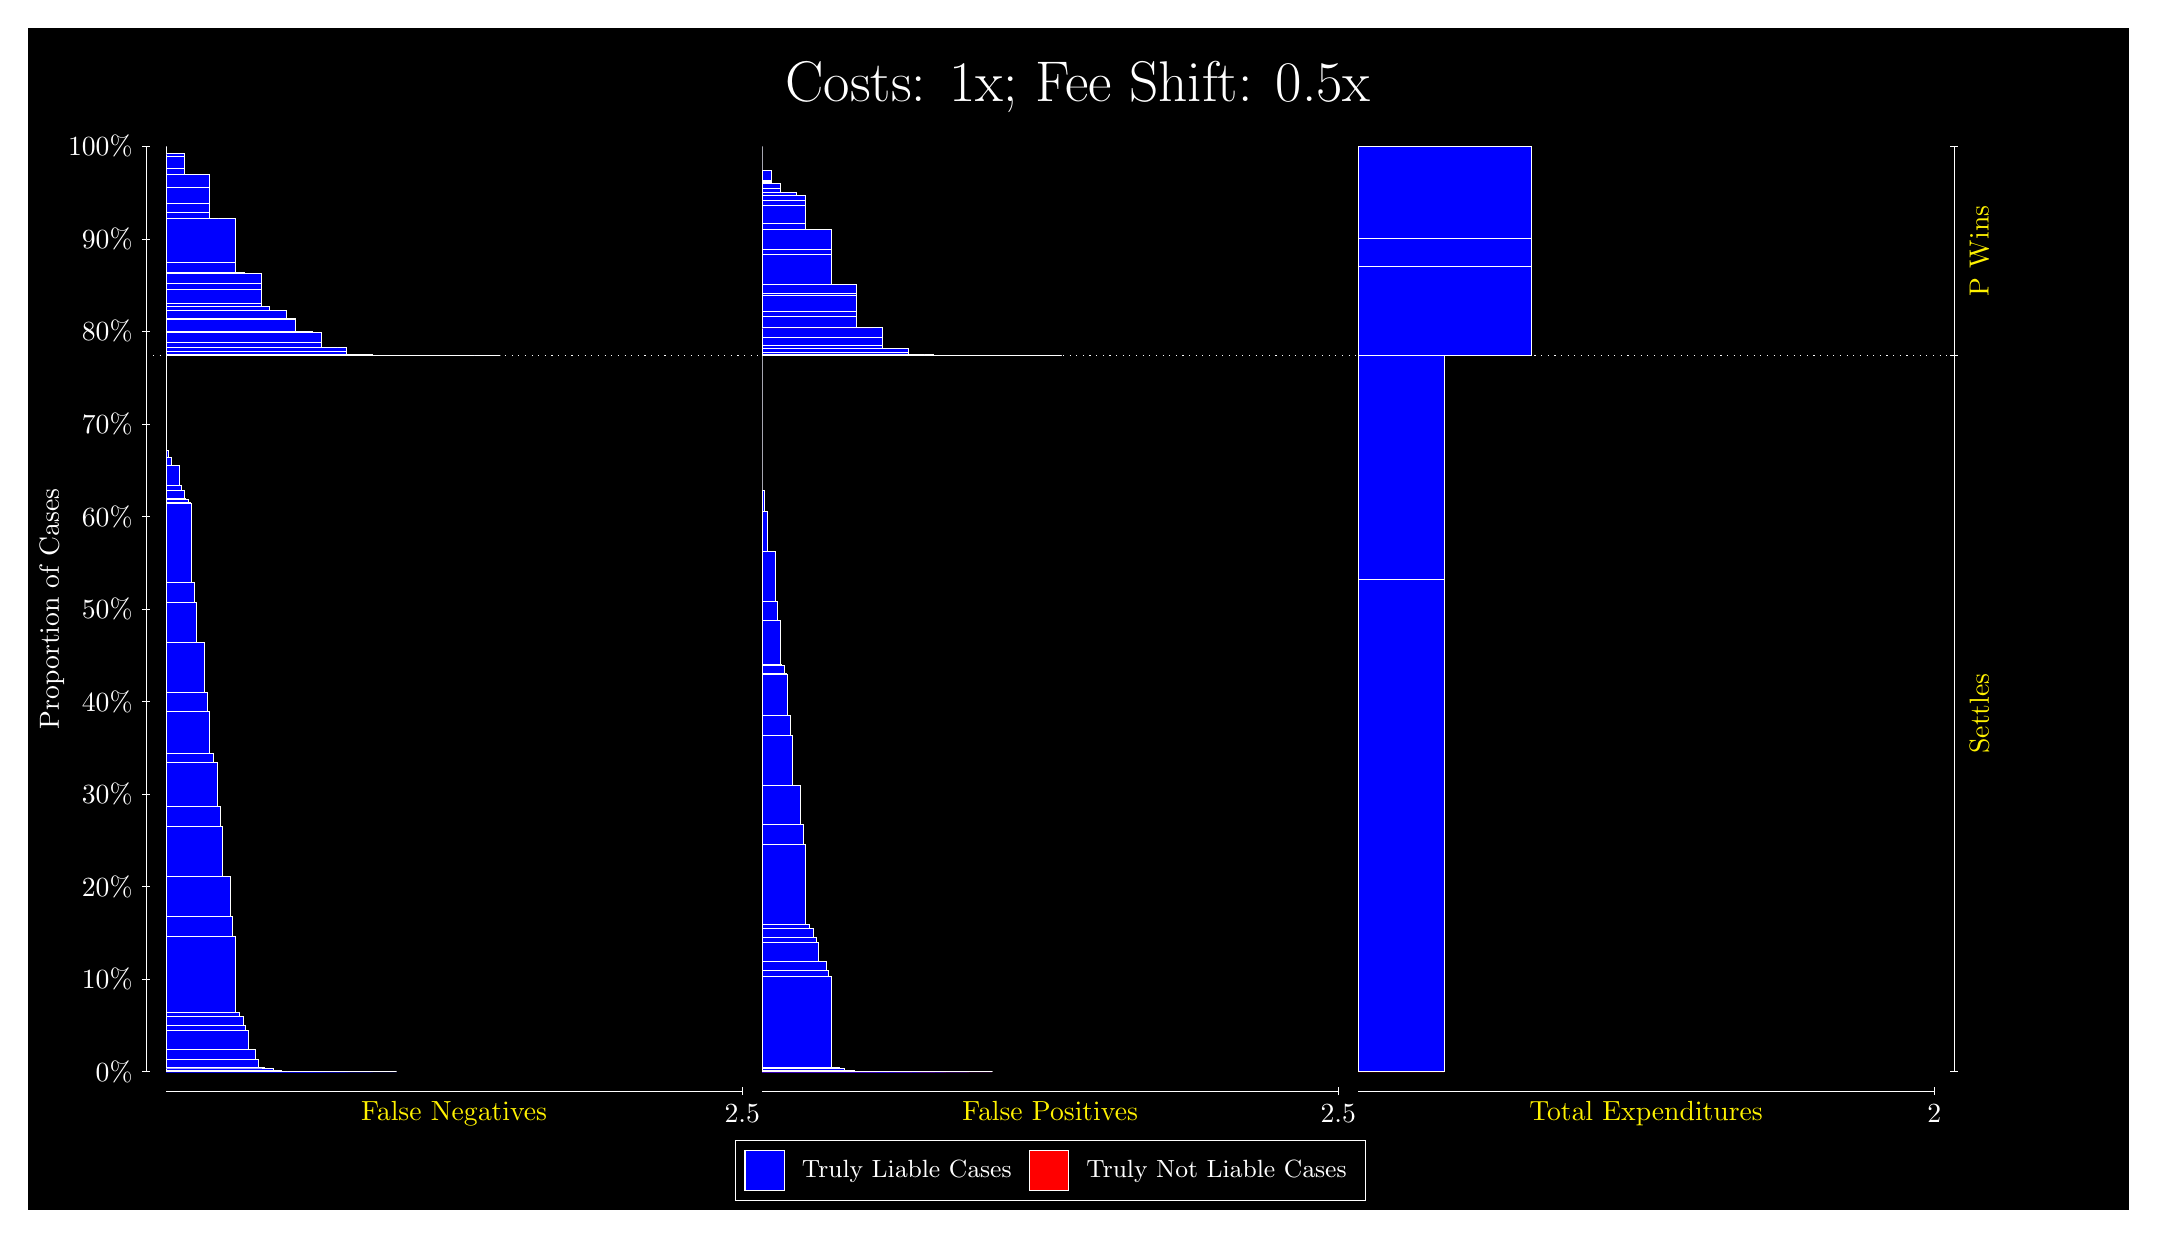
\begin{tikzpicture}
\draw[fill=black] (0,0) rectangle (26.667,15);
\draw[text=white] (0,13.5) rectangle (26.667,15) node[midway] {\huge Costs: 1x; Fee Shift: 0.5x};
\draw[white, very thin] (1.5,1.75) -- (1.5,13.5);
\node[rotate=90, text=white, anchor=center] at (0.3, 7.625) {Proportion of Cases};
\draw[white, very thin] (1.45,1.75) -- (1.55,1.75);
\node[text=white, anchor=east] at (1.45, 1.75) {0\%};
\draw[white, very thin] (1.45,2.925) -- (1.55,2.925);
\node[text=white, anchor=east] at (1.45, 2.925) {10\%};
\draw[white, very thin] (1.45,4.1) -- (1.55,4.1);
\node[text=white, anchor=east] at (1.45, 4.1) {20\%};
\draw[white, very thin] (1.45,5.275) -- (1.55,5.275);
\node[text=white, anchor=east] at (1.45, 5.275) {30\%};
\draw[white, very thin] (1.45,6.45) -- (1.55,6.45);
\node[text=white, anchor=east] at (1.45, 6.45) {40\%};
\draw[white, very thin] (1.45,7.625) -- (1.55,7.625);
\node[text=white, anchor=east] at (1.45, 7.625) {50\%};
\draw[white, very thin] (1.45,8.8) -- (1.55,8.8);
\node[text=white, anchor=east] at (1.45, 8.8) {60\%};
\draw[white, very thin] (1.45,9.975) -- (1.55,9.975);
\node[text=white, anchor=east] at (1.45, 9.975) {70\%};
\draw[white, very thin] (1.45,11.15) -- (1.55,11.15);
\node[text=white, anchor=east] at (1.45, 11.15) {80\%};
\draw[white, very thin] (1.45,12.325) -- (1.55,12.325);
\node[text=white, anchor=east] at (1.45, 12.325) {90\%};
\draw[white, very thin] (1.45,13.5) -- (1.55,13.5);
\node[text=white, anchor=east] at (1.45, 13.5) {100\%};

\draw[white, very thin] (24.457,1.75) -- (24.457,13.5);
\draw[white, very thin] (24.407,1.75) -- (24.507,1.75);
\node[anchor=west] at (24.407, 1.75) {};
\draw[white, very thin] (24.407,10.844) -- (24.507,10.844);
\node[anchor=west] at (24.407, 10.844) {};
\draw[white, very thin] (24.407,13.5) -- (24.507,13.5);
\node[anchor=west] at (24.407, 13.5) {};

\draw[white, very thin, fill=blue] (1.75,1.75) rectangle (4.6775,1.75);
\draw[white, very thin, fill=blue] (1.75,1.75) rectangle (4.3848,1.75);
\draw[white, very thin, fill=blue] (1.75,1.75) rectangle (4.3523,1.75);
\draw[white, very thin, fill=blue] (1.75,1.75) rectangle (4.092,1.75);
\draw[white, very thin, fill=blue] (1.75,1.75) rectangle (4.0595,1.75);
\draw[white, very thin, fill=blue] (1.75,1.75) rectangle (4.027,1.75);
\draw[white, very thin, fill=blue] (1.75,1.75) rectangle (3.9457,1.75);
\draw[white, very thin, fill=blue] (1.75,1.75) rectangle (3.7668,1.75);
\draw[white, very thin, fill=blue] (1.75,1.75) rectangle (3.7342,1.75);
\draw[white, very thin, fill=blue] (1.75,1.75) rectangle (3.7017,1.75);
\draw[white, very thin, fill=blue] (1.75,1.75) rectangle (3.6529,1.75);
\draw[white, very thin, fill=blue] (1.75,1.75) rectangle (3.6204,1.75);
\draw[white, very thin, fill=blue] (1.75,1.75) rectangle (3.4415,1.7505);
\draw[white, very thin, fill=blue] (1.75,1.7505) rectangle (3.4089,1.7506);
\draw[white, very thin, fill=blue] (1.75,1.7506) rectangle (3.3764,1.7506);
\draw[white, very thin, fill=blue] (1.75,1.7506) rectangle (3.3602,1.7506);
\draw[white, very thin, fill=blue] (1.75,1.7506) rectangle (3.3276,1.7507);
\draw[white, very thin, fill=blue] (1.75,1.7507) rectangle (3.2951,1.7507);
\draw[white, very thin, fill=blue] (1.75,1.7507) rectangle (3.2138,1.7617);
\draw[white, very thin, fill=blue] (1.75,1.7617) rectangle (3.1162,1.7858);
\draw[white, very thin, fill=blue] (1.75,1.7858) rectangle (3.0837,1.7908);
\draw[white, very thin, fill=blue] (1.75,1.7908) rectangle (3.0511,1.796);
\draw[white, very thin, fill=blue] (1.75,1.796) rectangle (3.0349,1.7962);
\draw[white, very thin, fill=blue] (1.75,1.7962) rectangle (3.0023,1.8008);
\draw[white, very thin, fill=blue] (1.75,1.8008) rectangle (2.9698,1.801);
\draw[white, very thin, fill=blue] (1.75,1.801) rectangle (2.921,1.9036);
\draw[white, very thin, fill=blue] (1.75,1.9036) rectangle (2.8885,2.0293);
\draw[white, very thin, fill=blue] (1.75,2.0293) rectangle (2.7909,2.2728);
\draw[white, very thin, fill=blue] (1.75,2.2728) rectangle (2.7584,2.3408);
\draw[white, very thin, fill=blue] (1.75,2.3408) rectangle (2.7258,2.4525);
\draw[white, very thin, fill=blue] (1.75,2.4525) rectangle (2.7096,2.4547);
\draw[white, very thin, fill=blue] (1.75,2.4547) rectangle (2.6771,2.5036);
\draw[white, very thin, fill=blue] (1.75,2.5036) rectangle (2.6445,2.5058);
\draw[white, very thin, fill=blue] (1.75,2.5058) rectangle (2.6283,3.4648);
\draw[white, very thin, fill=blue] (1.75,3.4648) rectangle (2.5957,3.7246);
\draw[white, very thin, fill=blue] (1.75,3.7246) rectangle (2.5632,4.2339);
\draw[white, very thin, fill=blue] (1.75,4.2339) rectangle (2.4656,4.8698);
\draw[white, very thin, fill=blue] (1.75,4.8698) rectangle (2.4331,5.1182);
\draw[white, very thin, fill=blue] (1.75,5.1182) rectangle (2.4006,5.6768);
\draw[white, very thin, fill=blue] (1.75,5.6768) rectangle (2.3843,5.682);
\draw[white, very thin, fill=blue] (1.75,5.682) rectangle (2.3518,5.7895);
\draw[white, very thin, fill=blue] (1.75,5.7895) rectangle (2.3192,5.7947);
\draw[white, very thin, fill=blue] (1.75,5.7947) rectangle (2.303,6.3212);
\draw[white, very thin, fill=blue] (1.75,6.3212) rectangle (2.2705,6.5677);
\draw[white, very thin, fill=blue] (1.75,6.5677) rectangle (2.2379,7.2039);
\draw[white, very thin, fill=blue] (1.75,7.2039) rectangle (2.1403,7.7071);
\draw[white, very thin, fill=blue] (1.75,7.7071) rectangle (2.1078,7.9584);
\draw[white, very thin, fill=blue] (1.75,7.9584) rectangle (2.0753,8.9712);
\draw[white, very thin, fill=blue] (1.75,8.9712) rectangle (2.059,8.9734);
\draw[white, very thin, fill=blue] (1.75,8.9734) rectangle (2.0265,9.0223);
\draw[white, very thin, fill=blue] (1.75,9.0223) rectangle (1.994,9.0245);
\draw[white, very thin, fill=blue] (1.75,9.0245) rectangle (1.9777,9.1333);
\draw[white, very thin, fill=blue] (1.75,9.1333) rectangle (1.9452,9.2011);
\draw[white, very thin, fill=blue] (1.75,9.2011) rectangle (1.9126,9.4445);
\draw[white, very thin, fill=blue] (1.75,9.4445) rectangle (1.8151,9.5554);
\draw[white, very thin, fill=blue] (1.75,9.5554) rectangle (1.7825,9.6335);
\draw[white, very thin, fill=red] (1.75,9.6335) rectangle (1.75,9.6335);
\draw[white, very thin, fill=blue] (1.75,9.6335) rectangle (1.75,10.844);
\draw[white, very thin, fill=blue] (1.75,10.844) rectangle (5.9949,10.844);
\draw[white, very thin, fill=blue] (1.75,10.844) rectangle (5.6697,10.844);
\draw[white, very thin, fill=blue] (1.75,10.844) rectangle (5.3444,10.844);
\draw[white, very thin, fill=blue] (1.75,10.844) rectangle (5.3444,10.844);
\draw[white, very thin, fill=blue] (1.75,10.844) rectangle (5.0191,10.844);
\draw[white, very thin, fill=blue] (1.75,10.844) rectangle (4.9052,10.844);
\draw[white, very thin, fill=blue] (1.75,10.844) rectangle (4.6938,10.846);
\draw[white, very thin, fill=blue] (1.75,10.846) rectangle (4.58,10.846);
\draw[white, very thin, fill=blue] (1.75,10.846) rectangle (4.58,10.846);
\draw[white, very thin, fill=blue] (1.75,10.846) rectangle (4.3685,10.864);
\draw[white, very thin, fill=blue] (1.75,10.864) rectangle (4.2547,10.864);
\draw[white, very thin, fill=blue] (1.75,10.864) rectangle (4.2547,10.864);
\draw[white, very thin, fill=blue] (1.75,10.864) rectangle (4.0432,10.895);
\draw[white, very thin, fill=blue] (1.75,10.895) rectangle (4.0432,10.947);
\draw[white, very thin, fill=blue] (1.75,10.947) rectangle (3.9294,10.947);
\draw[white, very thin, fill=blue] (1.75,10.947) rectangle (3.718,11.009);
\draw[white, very thin, fill=blue] (1.75,11.009) rectangle (3.718,11.14);
\draw[white, very thin, fill=blue] (1.75,11.14) rectangle (3.6041,11.149);
\draw[white, very thin, fill=blue] (1.75,11.149) rectangle (3.3927,11.303);
\draw[white, very thin, fill=blue] (1.75,11.303) rectangle (3.3927,11.314);
\draw[white, very thin, fill=blue] (1.75,11.314) rectangle (3.2788,11.315);
\draw[white, very thin, fill=blue] (1.75,11.315) rectangle (3.2788,11.422);
\draw[white, very thin, fill=blue] (1.75,11.422) rectangle (3.0674,11.466);
\draw[white, very thin, fill=blue] (1.75,11.466) rectangle (2.9535,11.501);
\draw[white, very thin, fill=blue] (1.75,11.501) rectangle (2.9535,11.687);
\draw[white, very thin, fill=blue] (1.75,11.687) rectangle (2.9535,11.756);
\draw[white, very thin, fill=blue] (1.75,11.756) rectangle (2.9535,11.894);
\draw[white, very thin, fill=blue] (1.75,11.894) rectangle (2.7421,11.898);
\draw[white, very thin, fill=blue] (1.75,11.898) rectangle (2.7421,11.898);
\draw[white, very thin, fill=blue] (1.75,11.898) rectangle (2.6283,12.022);
\draw[white, very thin, fill=blue] (1.75,12.022) rectangle (2.6283,12.591);
\draw[white, very thin, fill=blue] (1.75,12.591) rectangle (2.4168,12.591);
\draw[white, very thin, fill=blue] (1.75,12.591) rectangle (2.4168,12.591);
\draw[white, very thin, fill=blue] (1.75,12.591) rectangle (2.303,12.658);
\draw[white, very thin, fill=blue] (1.75,12.658) rectangle (2.303,12.777);
\draw[white, very thin, fill=blue] (1.75,12.777) rectangle (2.303,12.983);
\draw[white, very thin, fill=blue] (1.75,12.983) rectangle (2.303,13.147);
\draw[white, very thin, fill=blue] (1.75,13.147) rectangle (2.0915,13.147);
\draw[white, very thin, fill=blue] (1.75,13.147) rectangle (2.0915,13.147);
\draw[white, very thin, fill=blue] (1.75,13.147) rectangle (1.9777,13.226);
\draw[white, very thin, fill=blue] (1.75,13.226) rectangle (1.9777,13.374);
\draw[white, very thin, fill=blue] (1.75,13.374) rectangle (1.9777,13.408);
\draw[white, very thin, fill=blue] (1.75,13.408) rectangle (1.7663,13.408);
\draw[white, very thin, fill=blue] (1.75,13.408) rectangle (1.7663,13.408);
\draw[white, very thin, fill=red] (1.75,13.408) rectangle (1.75,13.408);
\draw[white, very thin, fill=blue] (1.75,13.408) rectangle (1.75,13.5);
\draw[white, very thin, fill=red] (9.3189,1.75) rectangle (12.246,1.75);
\draw[white, very thin, fill=blue] (9.3189,1.75) rectangle (12.246,1.75);
\draw[white, very thin, fill=red] (9.3189,1.75) rectangle (11.954,1.75);
\draw[white, very thin, fill=blue] (9.3189,1.75) rectangle (11.954,1.75);
\draw[white, very thin, fill=blue] (9.3189,1.75) rectangle (11.921,1.75);
\draw[white, very thin, fill=red] (9.3189,1.75) rectangle (11.661,1.75);
\draw[white, very thin, fill=blue] (9.3189,1.75) rectangle (11.661,1.75);
\draw[white, very thin, fill=blue] (9.3189,1.75) rectangle (11.628,1.75);
\draw[white, very thin, fill=blue] (9.3189,1.75) rectangle (11.596,1.75);
\draw[white, very thin, fill=red] (9.3189,1.75) rectangle (11.515,1.75);
\draw[white, very thin, fill=blue] (9.3189,1.75) rectangle (11.515,1.75);
\draw[white, very thin, fill=blue] (9.3189,1.75) rectangle (11.336,1.75);
\draw[white, very thin, fill=blue] (9.3189,1.75) rectangle (11.303,1.75);
\draw[white, very thin, fill=blue] (9.3189,1.75) rectangle (11.271,1.75);
\draw[white, very thin, fill=red] (9.3189,1.75) rectangle (11.222,1.75);
\draw[white, very thin, fill=blue] (9.3189,1.75) rectangle (11.222,1.75);
\draw[white, very thin, fill=blue] (9.3189,1.75) rectangle (11.189,1.75);
\draw[white, very thin, fill=blue] (9.3189,1.75) rectangle (11.01,1.75);
\draw[white, very thin, fill=blue] (9.3189,1.75) rectangle (10.978,1.75);
\draw[white, very thin, fill=blue] (9.3189,1.75) rectangle (10.945,1.75);
\draw[white, very thin, fill=red] (9.3189,1.75) rectangle (10.929,1.75);
\draw[white, very thin, fill=blue] (9.3189,1.75) rectangle (10.929,1.75);
\draw[white, very thin, fill=blue] (9.3189,1.75) rectangle (10.896,1.75);
\draw[white, very thin, fill=blue] (9.3189,1.75) rectangle (10.864,1.75);
\draw[white, very thin, fill=red] (9.3189,1.75) rectangle (10.783,1.75);
\draw[white, very thin, fill=blue] (9.3189,1.75) rectangle (10.783,1.7501);
\draw[white, very thin, fill=blue] (9.3189,1.7501) rectangle (10.685,1.7506);
\draw[white, very thin, fill=blue] (9.3189,1.7506) rectangle (10.653,1.7507);
\draw[white, very thin, fill=blue] (9.3189,1.7507) rectangle (10.62,1.7507);
\draw[white, very thin, fill=blue] (9.3189,1.7507) rectangle (10.604,1.7507);
\draw[white, very thin, fill=blue] (9.3189,1.7507) rectangle (10.571,1.7508);
\draw[white, very thin, fill=blue] (9.3189,1.7508) rectangle (10.539,1.7508);
\draw[white, very thin, fill=red] (9.3189,1.7508) rectangle (10.49,1.7508);
\draw[white, very thin, fill=blue] (9.3189,1.7508) rectangle (10.49,1.7613);
\draw[white, very thin, fill=blue] (9.3189,1.7613) rectangle (10.457,1.7673);
\draw[white, very thin, fill=blue] (9.3189,1.7673) rectangle (10.36,1.7914);
\draw[white, very thin, fill=blue] (9.3189,1.7914) rectangle (10.327,1.7964);
\draw[white, very thin, fill=blue] (9.3189,1.7964) rectangle (10.295,1.8016);
\draw[white, very thin, fill=blue] (9.3189,1.8016) rectangle (10.278,1.8018);
\draw[white, very thin, fill=blue] (9.3189,1.8018) rectangle (10.246,1.8063);
\draw[white, very thin, fill=blue] (9.3189,1.8063) rectangle (10.213,1.8065);
\draw[white, very thin, fill=red] (9.3189,1.8065) rectangle (10.197,1.8065);
\draw[white, very thin, fill=blue] (9.3189,1.8065) rectangle (10.197,2.9605);
\draw[white, very thin, fill=blue] (9.3189,2.9605) rectangle (10.165,3.0386);
\draw[white, very thin, fill=blue] (9.3189,3.0386) rectangle (10.132,3.1495);
\draw[white, very thin, fill=blue] (9.3189,3.1495) rectangle (10.034,3.3929);
\draw[white, very thin, fill=blue] (9.3189,3.3929) rectangle (10.002,3.4607);
\draw[white, very thin, fill=blue] (9.3189,3.4607) rectangle (9.9694,3.5694);
\draw[white, very thin, fill=blue] (9.3189,3.5694) rectangle (9.9532,3.5717);
\draw[white, very thin, fill=blue] (9.3189,3.5717) rectangle (9.9206,3.6206);
\draw[white, very thin, fill=blue] (9.3189,3.6206) rectangle (9.8881,3.6228);
\draw[white, very thin, fill=blue] (9.3189,3.6228) rectangle (9.8718,4.6356);
\draw[white, very thin, fill=blue] (9.3189,4.6356) rectangle (9.8393,4.8869);
\draw[white, very thin, fill=blue] (9.3189,4.8869) rectangle (9.8068,5.3901);
\draw[white, very thin, fill=blue] (9.3189,5.3901) rectangle (9.7092,6.0263);
\draw[white, very thin, fill=blue] (9.3189,6.0263) rectangle (9.6767,6.2728);
\draw[white, very thin, fill=blue] (9.3189,6.2728) rectangle (9.6442,6.7993);
\draw[white, very thin, fill=blue] (9.3189,6.7993) rectangle (9.6279,6.8045);
\draw[white, very thin, fill=blue] (9.3189,6.8045) rectangle (9.5954,6.9119);
\draw[white, very thin, fill=blue] (9.3189,6.9119) rectangle (9.5628,6.9172);
\draw[white, very thin, fill=blue] (9.3189,6.9172) rectangle (9.5466,7.4758);
\draw[white, very thin, fill=blue] (9.3189,7.4758) rectangle (9.514,7.7242);
\draw[white, very thin, fill=blue] (9.3189,7.7242) rectangle (9.4815,8.3601);
\draw[white, very thin, fill=blue] (9.3189,8.3601) rectangle (9.3839,8.8693);
\draw[white, very thin, fill=blue] (9.3189,8.8693) rectangle (9.3514,9.1292);
\draw[white, very thin, fill=blue] (9.3189,9.1292) rectangle (9.3189,10.844);
\draw[white, very thin, fill=red] (9.3189,10.844) rectangle (13.125,10.844);
\draw[white, very thin, fill=blue] (9.3189,10.844) rectangle (13.125,10.844);
\draw[white, very thin, fill=red] (9.3189,10.844) rectangle (12.799,10.844);
\draw[white, very thin, fill=blue] (9.3189,10.844) rectangle (12.799,10.844);
\draw[white, very thin, fill=blue] (9.3189,10.844) rectangle (12.474,10.844);
\draw[white, very thin, fill=red] (9.3189,10.844) rectangle (12.474,10.844);
\draw[white, very thin, fill=blue] (9.3189,10.844) rectangle (12.474,10.844);
\draw[white, very thin, fill=blue] (9.3189,10.844) rectangle (12.149,10.844);
\draw[white, very thin, fill=blue] (9.3189,10.844) rectangle (12.149,10.844);
\draw[white, very thin, fill=red] (9.3189,10.844) rectangle (12.149,10.844);
\draw[white, very thin, fill=blue] (9.3189,10.844) rectangle (12.149,10.844);
\draw[white, very thin, fill=red] (9.3189,10.844) rectangle (11.824,10.844);
\draw[white, very thin, fill=blue] (9.3189,10.844) rectangle (11.824,10.845);
\draw[white, very thin, fill=blue] (9.3189,10.845) rectangle (11.824,10.845);
\draw[white, very thin, fill=blue] (9.3189,10.845) rectangle (11.824,10.845);
\draw[white, very thin, fill=red] (9.3189,10.845) rectangle (11.498,10.845);
\draw[white, very thin, fill=blue] (9.3189,10.845) rectangle (11.498,10.857);
\draw[white, very thin, fill=blue] (9.3189,10.857) rectangle (11.498,10.859);
\draw[white, very thin, fill=red] (9.3189,10.859) rectangle (11.384,10.859);
\draw[white, very thin, fill=blue] (9.3189,10.859) rectangle (11.384,10.859);
\draw[white, very thin, fill=blue] (9.3189,10.859) rectangle (11.173,10.884);
\draw[white, very thin, fill=red] (9.3189,10.884) rectangle (11.173,10.884);
\draw[white, very thin, fill=blue] (9.3189,10.884) rectangle (11.173,10.936);
\draw[white, very thin, fill=blue] (9.3189,10.936) rectangle (11.059,10.936);
\draw[white, very thin, fill=red] (9.3189,10.936) rectangle (11.059,10.936);
\draw[white, very thin, fill=blue] (9.3189,10.936) rectangle (11.059,10.936);
\draw[white, very thin, fill=blue] (9.3189,10.936) rectangle (10.848,10.97);
\draw[white, very thin, fill=blue] (9.3189,10.97) rectangle (10.848,11.079);
\draw[white, very thin, fill=red] (9.3189,11.079) rectangle (10.848,11.079);
\draw[white, very thin, fill=blue] (9.3189,11.079) rectangle (10.848,11.197);
\draw[white, very thin, fill=blue] (9.3189,11.197) rectangle (10.734,11.197);
\draw[white, very thin, fill=blue] (9.3189,11.197) rectangle (10.734,11.197);
\draw[white, very thin, fill=red] (9.3189,11.197) rectangle (10.734,11.197);
\draw[white, very thin, fill=blue] (9.3189,11.197) rectangle (10.734,11.197);
\draw[white, very thin, fill=blue] (9.3189,11.197) rectangle (10.522,11.344);
\draw[white, very thin, fill=blue] (9.3189,11.344) rectangle (10.522,11.409);
\draw[white, very thin, fill=blue] (9.3189,11.409) rectangle (10.522,11.614);
\draw[white, very thin, fill=blue] (9.3189,11.614) rectangle (10.522,11.634);
\draw[white, very thin, fill=blue] (9.3189,11.634) rectangle (10.522,11.753);
\draw[white, very thin, fill=blue] (9.3189,11.753) rectangle (10.409,11.753);
\draw[white, very thin, fill=red] (9.3189,11.753) rectangle (10.409,11.753);
\draw[white, very thin, fill=blue] (9.3189,11.753) rectangle (10.409,11.753);
\draw[white, very thin, fill=blue] (9.3189,11.753) rectangle (10.409,11.753);
\draw[white, very thin, fill=blue] (9.3189,11.753) rectangle (10.197,12.126);
\draw[white, very thin, fill=blue] (9.3189,12.126) rectangle (10.197,12.192);
\draw[white, very thin, fill=blue] (9.3189,12.192) rectangle (10.197,12.446);
\draw[white, very thin, fill=blue] (9.3189,12.446) rectangle (10.083,12.446);
\draw[white, very thin, fill=blue] (9.3189,12.446) rectangle (10.083,12.446);
\draw[white, very thin, fill=red] (9.3189,12.446) rectangle (10.083,12.446);
\draw[white, very thin, fill=blue] (9.3189,12.446) rectangle (10.083,12.45);
\draw[white, very thin, fill=blue] (9.3189,12.45) rectangle (9.8718,12.522);
\draw[white, very thin, fill=blue] (9.3189,12.522) rectangle (9.8718,12.757);
\draw[white, very thin, fill=blue] (9.3189,12.757) rectangle (9.8718,12.81);
\draw[white, very thin, fill=blue] (9.3189,12.81) rectangle (9.8718,12.878);
\draw[white, very thin, fill=blue] (9.3189,12.878) rectangle (9.758,12.879);
\draw[white, very thin, fill=red] (9.3189,12.879) rectangle (9.758,12.879);
\draw[white, very thin, fill=blue] (9.3189,12.879) rectangle (9.758,12.883);
\draw[white, very thin, fill=blue] (9.3189,12.883) rectangle (9.758,12.921);
\draw[white, very thin, fill=blue] (9.3189,12.921) rectangle (9.5466,12.969);
\draw[white, very thin, fill=blue] (9.3189,12.969) rectangle (9.5466,13.03);
\draw[white, very thin, fill=blue] (9.3189,13.03) rectangle (9.4327,13.04);
\draw[white, very thin, fill=blue] (9.3189,13.04) rectangle (9.4327,13.052);
\draw[white, very thin, fill=blue] (9.3189,13.052) rectangle (9.4327,13.072);
\draw[white, very thin, fill=blue] (9.3189,13.072) rectangle (9.4327,13.194);
\draw[white, very thin, fill=blue] (9.3189,13.194) rectangle (9.3189,13.5);
\draw[white, very thin, fill=red] (16.888,1.75) rectangle (17.986,1.75);
\draw[white, very thin, fill=blue] (16.888,1.75) rectangle (17.986,8.0015);
\draw[white, very thin, fill=red] (16.888,8.0015) rectangle (17.986,8.0015);
\draw[white, very thin, fill=blue] (16.888,8.0015) rectangle (17.986,10.844);
\draw[white, very thin, fill=red] (16.888,10.844) rectangle (19.083,10.844);
\draw[white, very thin, fill=blue] (16.888,10.844) rectangle (19.083,11.974);
\draw[white, very thin, fill=red] (16.888,11.974) rectangle (19.083,11.974);
\draw[white, very thin, fill=blue] (16.888,11.974) rectangle (19.083,12.332);
\draw[white, very thin, fill=red] (16.888,12.332) rectangle (19.083,12.332);
\draw[white, very thin, fill=blue] (16.888,12.332) rectangle (19.083,13.5);
\draw[white, dotted] (1.5,10.844) -- (24.457,10.844);
\draw[white, very thin] (1.75,1.5) -- (9.0689,1.5);
\node[text=yellow, anchor=north] at (5.4094, 1.5) {False Negatives};
\draw[white, very thin] (9.0689,1.45) -- (9.0689,1.55);
\node[text=white, anchor=north] at (9.0689, 1.45) {2.5};

\draw[white, very thin] (9.3189,1.5) -- (16.638,1.5);
\node[text=yellow, anchor=north] at (12.978, 1.5) {False Positives};
\draw[white, very thin] (16.638,1.45) -- (16.638,1.55);
\node[text=white, anchor=north] at (16.638, 1.45) {2.5};

\draw[white, very thin] (16.888,1.5) -- (24.207,1.5);
\node[text=yellow, anchor=north] at (20.547, 1.5) {Total Expenditures};
\draw[white, very thin] (24.207,1.45) -- (24.207,1.55);
\node[text=white, anchor=north] at (24.207, 1.45) {2};

\node[text=yellow, centered, rotate=90] at (24.777, 6.297) {Settles};
\node[text=yellow, centered, rotate=90] at (24.777, 12.172) {P Wins};

\draw (12.978300999999998,1.5) node[draw=none] (baseCoordinate) {};
\begin{scope}[align=center]
        \matrix[scale=0.5, draw=white, below=0.5cm of baseCoordinate, nodes={draw}, column sep=0.1cm]{
            \node[rectangle, draw, minimum width=0.5cm, minimum height=0.5cm, fill=blue] {}; &
            \node[draw=none, font=\small, text=white] (B) {Truly Liable Cases}; &
            \node[rectangle, draw, minimum width=0.5cm, minimum height=0.5cm, fill=red] {}; &
            \node[draw=none, font=\small, text=white] (B) {Truly Not Liable Cases}; \\
            };
\end{scope}

\end{tikzpicture}
\end{document}